%!TEX root = main.tex
\begin{figure*}[t]
\centering
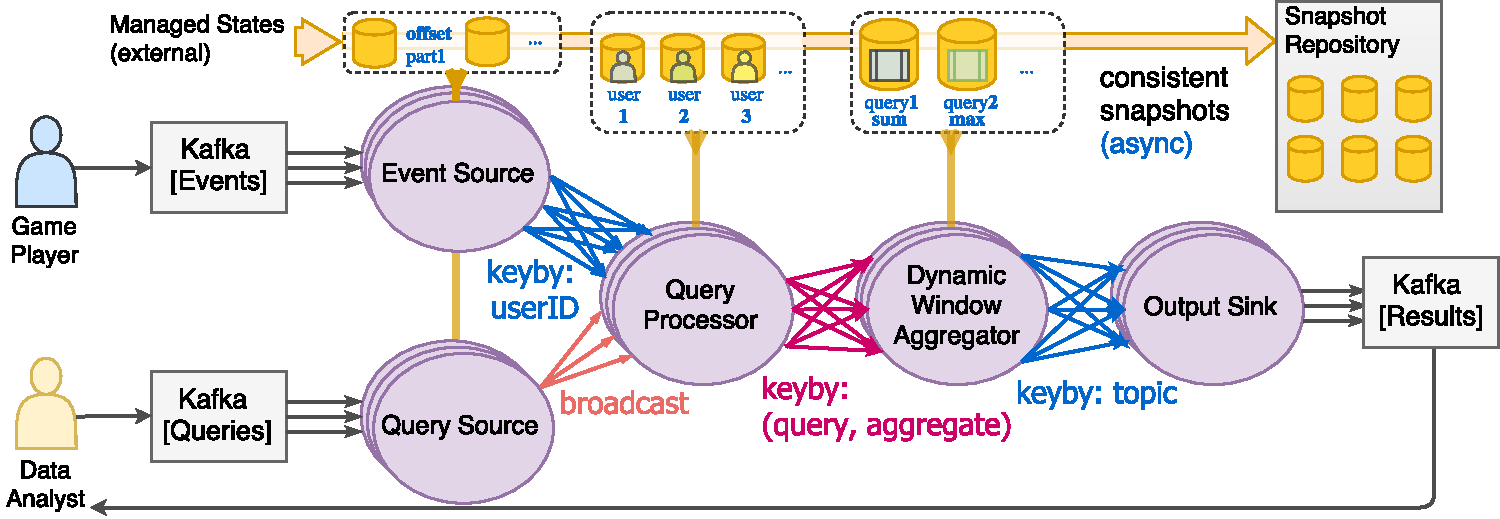
\includegraphics[width=\textwidth]{figures/rbea.pdf}
\caption{A Flink pipeline implementing an adhoc standing query execution service (King AB)} 
\label{fig:rbea}
\vspace{-4mm}
\end{figure*}

\section{Large-Scale Deployments}
\label{sec:evaluation}


Flink is currently one of the most widespread systems in production\gyula{is this claim true?}, serving as a the core engine for continuous data processing. Large-scale deployments range from dozens to 1000s of nodes and serve a wide variety of data management and analysis needs. In this section, we present a few examples of how Flink's lightweight state management features are being used in practice, within large deployments and also present live metrics and insights.

\paris{we can either divide use cases by topic or by company. I am a bit in favor of topic-based. E.g. 1) Flink as a Distributed Dynamic Data Index (Alibaba), 2) Flink as a Standing Query Execution Engine (King), etc. @Kostas feel free to add whatever text and refs you like in this section. No need to add your tag. I can see the diffs in sharelatex and do another pass afterwards}

\para{Alibaba} is actively using Flink in their production cluster (1000+ nodes) to support their critical search service \cite{CUSTOM:web/alibaba} and keep search results and recommendation as fresh and relevant to their active retail catalogue as possible.

%King.com

%\para{Zalando}

%\para{Uber}


%\para{Bouygues Telecom}

%\para{ResearchGate}

%Uber, Netflix, ING, MediaMath, New Relic



\subsection{A Real-Time Analytics Platform}

The Rule-Based Event Aggregator (RBEA) by King AB \cite{CUSTOM:web/kingrbea}, is a reliable live service that is implemented on Apache Flink and used daily by data analysts and database engineers for more than a year. RBEA showcases how Flink's stateful processing capabilities can be exploited to build a highly dynamic live service that allows analysts to declare and run standing queries on large-scale mobile event streams, backed by Flink's consistent state. In essence, the service covers several fundamental needs of data analysts: 1) instant access to timely user data, 2) the ability to deploy declarative standing queries, 3) creation and manipulation of custom aggregation metrics, 4) a transparent execution, eliminating the need for technical expertise.

\autoref{fig:rbea} depicts an overview of the end-to-end Flink pipeline that implements the core of the service. There are two types of streams, ingested from Kafka: a) an \texttt{Event} stream originating from  user actions (circa 30 billion events per day) such as \texttt{GameStarted} or \texttt{GameEnded} and b) a \texttt{Query} stream containing standing queries in the form of serialized scripts written by data analysts through the frontend of RBEA in a provided DSL (e.g., using Groovy or Java). Standing queries in RBEA allow analysts to access user-specific data and event sequences as well as triggering special aggregation logic on sliding data windows (respecting the semantics of Flink's implementation of the Dataflow Model \cite{akidau2015dataflow}). 

The user defined queries are stored and executed inside the [Query Processor] operator which holds the user states accumulated by any stateful processing logic. Every user query is broadcasted to all instances of the [Query Processor] so it can be executed in parallel while game events are partitioned by their associated user ids. Aggregation calls in the RBEA DSL trigger output events from [Query Processor] operator which are subsequently consumed by the [Dynamic Window Aggregator]. This operator assigns the aggregator events to the current event-time window and does the actual aggregation. Aggregated values are sent to the [Output sink] operator which writes them to an external database or Kafka.

%failures during script execution need to be backpropagated to all the parallel instances in order the remove all instances of the broken scripts. Iterations are used to implement the failure propagation logic.


from the along with the different types of states associated with each operator.

\par{Performance Metrics:} The performance of the state management layer have been evaluated along multiple dimensions:
\begin{itemize}
    \item With fixed parallelism measure total checkpoint and alignment time against state size
    \item With fixed state size measure total checkpoint and alignment time against parallelism
\end{itemize}

%130 - script engine 
%390 - aggregations
%404 - kafka output

